\section{Aufgabe 6}
F"ur die Expansion einer Supernova-Blase in der Sedov-Taylor Phase gilt:
\begin{equation}
R_{SNR,II}(t)=R_I + \left( 2.02 \frac{E_{SN}}{\rho_0} \right) ^{1/5}(t-t_1)^{2/5}
\end{equation}
\begin{tabular}{l l}
\(R_{SNR,II}(t)\)&\(\dots\) Expansionsradius in \(m\)\\
\(R_I\)&\(\dots\) Expansionsradius am Beginn der Phase in \(m\)\\
\(E_SN\)&\(\dots\) Explosionsenergie in \(J\)\\
\(\rho_0\)&\(\dots\) Umgebungsdichte in \(kg \cdot m^{-3}\)\\
\(t\)&\(\dots\) Dauer der Expansion in \(s\)\\
\(t_I\)&\(\dots\) Zeit die bis zum Beginn der Phase vergangen ist in \(s\)\\
\end{tabular}\\
\\
F"ur die Expansionsgeschwindigkeit gilt:
\begin{equation}
u_{SN,II}(t) = \frac{dR_{SNR,II}(t)}{dt}=\frac{2 \cdot 2.02^{1/5} \left( \frac{E_{SN}}{\rho_0} \right) ^{1/5}}{5(t-t_1)^{3/5}}
\end{equation}
Diese beiden Ausdr"ucke sind nun f"ur folgende Werte  zu berechnen:\\
\(E_{SN}=(0.5,1.0,2.0) \times 10^{51}~ergs = (0.5,1.0,2.0) \times 10^{44}~J\)\\
\(n_0=(0.01,1.0,100)~cm^{-3}\)\\
\(t_I=400~years=1.261 \times 10^{10}~s\)\\
\\
\(n_0\dots\) Umgebungsdichte in Teilchen pro \(cm^3\)\\
\\
F"ur die Berechnung von \(\rho_0\) wird die Masse von Wasserstoff (\(m_H=1.674 \times 10^{-27}~kg\)) verwendet:
\begin{equation}
\rho_0=n_0 \cdot m_H=(0.0167,1.674,167.37) \times 10^{-21}~kg \cdot m^{-3}
\end{equation}
\(R_I\) soll durch eine Expansion mit \(5000~km \cdot s^{-1}\) erreicht werden:
\begin{equation}
R_I=1.261 \times 10^{10}~s \cdot 5000~km \cdot s^{-1} = 6.3072 \times 10^{13} km
\end{equation}
\\
Ergebnisse in $Meter \times 10^{17}$:
\begin{center}
\begin{tabular}{|r|l|l|l|l|l|l|l|l|l|}
\multicolumn{10}{c}{\(R_{SNR,II}(t)\)}\\
\hline
\(n_0\) & \multicolumn{3}{|c|}{0.01} & \multicolumn{3}{|c|}{1.0} & \multicolumn{3}{|c|}{100}\\
\hline
\(E_{SN}~[erg]\) & 0.5 & 1.0 & 2.0 & 0.5 & 1.0 & 2.0 & 0.5 & 1.0 & 2.0\\
\hline
\(t~[10^{10}~s]\) & & & & & & & & & \\
\cline{1-1}
2 & $2.6$ & $2.9$ & $3.3$ &
$1.4$ & $1.5$ & $1.7$ &
$0.95$ & $1$ & $1.1$ \\

4 & $4$ & $4.5$ & $5.1$ &
$2$ & $2.2$ & $2.4$ &
$1.2$ & $1.2$ & $1.3$ \\

6 & $4.9$ & $5.5$ & $6.2$ &
$2.3$ & $2.6$ & $2.8$ &
$1.3$ & $1.4$ & $1.5$\\

8 & $5.5$ & $6.2$ & $7$ &
$2.6$ & $2.9$ & $3.2$ &
$1.4$ & $1.5$ & $1.6$\\

10 & $6$ & $6.8$ & $7.8$ &
$2.8$ & $3.1$ & $3.5$ &
$1.5$ & $1.6$ & $1.8$ \\

12 & $6.5$ & $7.4$ & $8.4$&
$3$ & $3.3$ & $3.7$ &
$1.6$ & $1.7$ & $1.9$ \\

\hline
\end{tabular}\\
\end{center}
\begin{figure}[ht]
\begin{center}
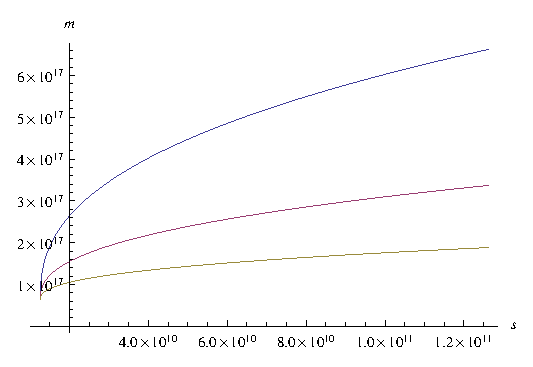
\includegraphics{aufgabe6r.eps}
\end{center}
\caption[Bildunterschrift]{Blau:n=0.01,EFaktor=0.5; Lila:n=1,EFaktor=1; Gelb:n=100;EFaktor=2;}
\end{figure}
Ergebnisse in $m/s \times 10^{6}$:
\begin{center}
\begin{tabular}{|r|l|l|l|l|l|l|l|l|l|}
\multicolumn{10}{c}{\(u_{SN,II}(t)\)}\\
\hline
\(n_0\) & \multicolumn{3}{|c|}{0.01} & \multicolumn{3}{|c|}{1.0} & \multicolumn{3}{|c|}{100}\\
\hline
\(E_{SN}~[erg]\) & 0.5 & 1.0 & 2.0 & 0.5 & 1.0 & 2.0 & 0.5 & 1.0 & 2.0\\
\hline
\(t~[10^{10}~s]\) & & & & & & & & & \\
\cline{1-1}
%1 & & & & & & & & & \\
2 & 11.1 & 12.5 & 14.3 &
4.3 & 5 & 5.7 &
1.7 & 2 & 2.3 \\

4 & 5 & 5.7 & 6.6 &
2 & 2.3 & 2.6 &
0.8 & 0.9 & 1 \\

6 & 3.6 & 4.1 & 4.7 &
1.4 & 1.6 & 1.9 &
0.6 & 0.7 & 0.7 \\

8 & 2.9 & 3.3 & 3.8 &
1.2 & 1.3 & 1.5 &
0.5 & 0.5 & 0.6 \\

10 & 2.5 & 2.8 & 3.3 &
1 & 1.1 & 1.3 &
0.4 & 0.5 & 0.5 \\

12 & 2.2 & 2.5 & 2.9 &
0.9 & 1 & 1.1 &
0.3 & 0.4 & 0.5 \\
\hline
\end{tabular}\\
\end{center}
\begin{figure}[ht]
\begin{center}
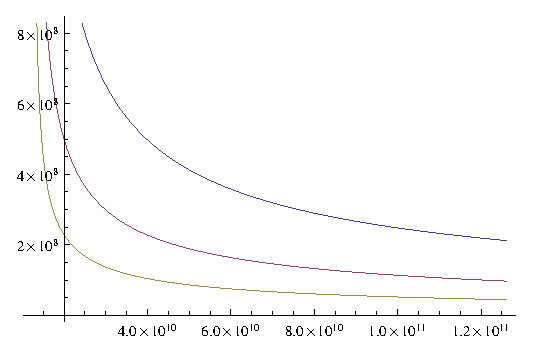
\includegraphics{aufgabe6u.eps}
\end{center}
\caption[Bildunterschrift]{Blau:n=0.01,EFaktor=0.5; Lila:n=1,EFaktor=1; Gelb:n=100;EFaktor=2;}
\end{figure}
